% !TEX recipe = pdfLaTeX

%%%%%%%%%%%%%%%%%%%%%%%%%%%%%%%%%%%%%%%%%%%%%%%%%%%%%%%%%%%
% LaTeX Template ~ 'tau-book.tex'
% Version 2.2 (15/03/2024)
%
% Description: 
% Tau-book is a LaTeX template that offers a clean and 
% professional design for lab reports or academic papers.
% The clarity of the code structure makes it easy to 
% understand and modify for your needs. This template uses 
% an easy-to-read font and high quality equations with "stix2".
%
% Author: 
% Guillermo Jimenez (memo.notess1@gmail.com)
% 
% License:
% Creative Commons CC BY 4.0
%%%%%%%%%%%%%%%%%%%%%%%%%%%%%%%%%%%%%%%%%%%%%%%%%%%%%%%%%%%
%     BIBLIOGRAPHY WITH BIBLATEX IN EXTERNAL EDITORS:
% If the bibliography does not show up, try running the 
% 'tau-book.cls' and 'tau.bib' file with biber from the 
% MikTeX console or your preferred LaTeX distribution to 
% generate the .aux files and (re)run tau-book.tex.
%%%%%%%%%%%%%%%%%%%%%%%%%%%%%%%%%%%%%%%%%%%%%%%%%%%%%%%%%%%

\documentclass[10pt,a4paper,twoside]{tau-book}
\usepackage[italian]{babel}
\usepackage{tau}

%----------------------------------------------------------
% Figure
%----------------------------------------------------------
% Le figure sono quelle generate da ../grafici.Rmd e salvate in
% ../figures/: vengono lette direttamente dalla cartella principale
% del progetto, senza mantenerne una copia locale.

\graphicspath{{../}{./}}

%----------------------------------------------------------
% Title
%----------------------------------------------------------

\title{Sul funzionamento dell'algoritmo di Strassen per matrici rettangolari}

\author{Luca Varotto}
\affil{Corso di Laurea in Statistica per le Tecnologie e le Scienze - Esame di Sistemi di Elaborazione 2}

% Richiesto da tau-book.cls, che usa \@professor nel titolo:
% lasciare vuoto per non stampare alcuna riga.
\professor{}

%----------------------------------------------------------
% Footpage notes
%----------------------------------------------------------

\institution{Università degli studi di Padova}
\ftitle{Report sul funzionamento dell'algoritmo di Strassen per matrici rettangolari}
\theday{\today}
\course{Esame di Sistemi di Elaborazione 2}

%----------------------------------------------------------

\begin{document}
	
\maketitle

\section{Introduzione}

Nel 1969 V. Strassen presentò un innovativo algoritmo per ridurre la complessità asintotica del calcolo matriciale da $O(n^3)$ a $O(n^{log_27})$, dove $log_27\approxeq2.807$ [1]. Questo miglioramento asintotico, è stato possibile grazie alla riduzione del numero di prodotti necessari nel moltiplicare tra loro due matrici di dimensioni $[2\times 2]$, in particolare i prodotti necessari furono ridotti da 8 a 7. Ad oggi questo algoritmo non è il più veloce per eseguire il prodotto riga per colonna, ma rimane fondamentale perché a partire da questo risultato sono stati sviluppati i successivi algoritmi, ancora più complessi, che hanno velocizzato ulteriormente il calcolo matriciale.

Nonostante il grande vantaggio asintotico presentato in precedenza, l'algoritmo di Strassen è stato a lungo trascurato, questo avvenne a causa di preoccupazioni legate alla sua presunta instabilità numerica e alla convinzione che diventasse vantaggioso solo per matrici di dimensioni superiori a $1000 \times 1000$. Tuttavia, nel 1990 [2], queste affermazioni sono state smentite, facendo ritornare in voga questo algoritmo.

Ad oggi, rimangono ancora due principali problematiche legate ad ogni implementazione possibile dell'algoritmo di Strassen:
\begin{enumerate}
    \item La scelta del "crossover point" Q, ovvero il valore soglia delle dimensioni delle matrici, che indica quando è conveniente passare dall'utilizzo dell'algoritmo di Strassen al classico prodotto riga per colonna.
    \item Lo sviluppo di un approccio che consenta di partizionare le matrici a blocchi utilizzando la minor quantità di memoria possibile.
\end{enumerate}
In questo breve report, verranno descritte quattro implementazioni dell'algoritmo di Strassen, con un focus particolare sulle tre per matrici rettangolari. Si discuterà inoltre, basandosi sulla letteratura esistente, della scelta del "crossover point" e di strategie per gestire efficientemente la memoria. Infine, si cercheranno di individuare ulteriori criticità e di proporre idee per una moderna implementazione dell'algoritmo. \\

Poiché tutte le conclusioni sono fortemente influenzate dai sistemi adottati, nel seguito verranno elencate le caratteristiche dell'hardware e del software utilizzati:
\begin{itemize}
    \item  Processore: Intel(R) Core(TM) i5-6300U CPU @ 2.40GHz (2.50 GHz)
    \item RAM: 16 GB
    \item Sistema operativo: 64 bit
    \item Linguaggio di programmazione: Python 3.12.2
    \item Libreria per la manipolazione delle matrici: NumPy 1.26.4
    \item Funzione per il calcolo del prodotto riga per colonna, dalla libreria numpy: numpy.matmul()
\end{itemize}

Per la generazione dei numeri pseudo-casuali, è stata utilizzata la libreria random. Prima di ogni generazione di numeri casuali è stato impostato un "seed", al fine di agevolare la replicabilità dei risultati. Per alleggerire la lettura, nelle sezioni seguenti ci si riferirà ai valori pseudo-casuali generati con la libreria random con il termine "numeri casuali".


\section{La versione originale dell'algoritmo}

Come introdotto in precedenza, la prima versione dell'algoritmo offriva una soluzione per moltiplicare una matrice A, di dimensioni $[j\times j]$, con una matrice B, di dimensioni $[j\times j]$, dove j è una potenza intera di 2, in modo da ottenere la matrice C, di dimensioni $[j\times j]$. In particolare, partizionando le matrici A e B in quattro blocchi di ugual dimensioni, ricaviamo che:
\begin{equation}
    \begin{bmatrix} C_{11} & C_{12} \\ C_{21} & C_{22} \end{bmatrix} = \begin{bmatrix} A_{11} & A_{12} \\ A_{21} & A_{22} \end{bmatrix} \begin{bmatrix} B_{11} & B_{12} \\ B_{21} & B_{22} \end{bmatrix}
\end{equation}
se definiamo le quantità:
\begin{equation}
\begin{aligned}
    M_1 =& (A_{11}+A_{22})(B_{11}+B_{12}) \\
    M_2 =& (A_{21}+A_{22})(B_{11}) \\
    M_3 =& (A_{11})(B_{12}-B_{22}) \\
    M_4 =& (A_{22})(B_{21}-B_{11}) \\
    M_5 =& (A_{11}+A_{12})(B_{22}) \\
    M_6 =& (A_{21}-A_{11})(B_{11}+B_{12}) \\
    M_7 =& (A_{12}-A_{22})(B_{11}+B_{22}) \\
\end{aligned}
\end{equation}
possiamo trovare che:
\begin{equation}
\label{eq:strassen_sums}
\begin{aligned}
    C_{11} =& M_1 + M_4 - M_5 + M_7 \\
    C_{12} =& M_1 + M_5 \\
    C_{21} =& M_2 + M_4 \\
    C_{22} =& M_1 + M_3 - M_2 + M_6
\end{aligned}
\end{equation}
in tal modo si riesce ad eseguire il prodotto tra due matrici di dimensioni $[2\times 2]$, riducendo il numero di prodotti necessari da 8 a 7. Tale algoritmo è stato implementato in Python con la funzione \textbf{Strassen\_squareM(A,B,Q)}, dove Q indica il "cross-over point". Si raggiunge il "cross-over point" quando almeno una delle dimensioni è minore o uguale a Q. Di default Q è uguale a 2, in questo modo si affronteranno tutte le moltiplicazioni possibili con l'algoritmo di Strassen. \\
Questa versione, che d'ora in avanti verrà detta "versione originale", ha purtroppo diversi limiti, uno dei più evidenti è che non permetta di eseguire il prodotto tra matrici rettangolari. Nella sezione \ref{sec:strassen_odd_matrix} vedremo come risolvere questo problema.

\subsection{Funzioni ausiliarie}
\label{subsec:funzioni_ausiliarie_square_strassen}

Le seguenti funzioni sono state implementate per migliorare la sintassi e per semplificare l’implementazione di \textbf{Strassen\_squareM(A,B,Q)}:

\begin{itemize}
    \item \textbf{split\_matrix(M)}: funzione che divide la matrice M in 4 blocchi, distribuiti su due righe e due colonne. Ciascun blocco avrà lo stesso numero di righe e di colonne.
    \item \textbf{merge\_matrix(M11, M12, M21, M22)}: funzione che dati i 4 blocchi di una matrice, distribuiti su due righe e su due colonne, ne restituisce la loro composizione.
    \item \textbf{merge\_sums(M1, M2, M3, M4, M5, M6, M7)}: funzione per trovare i quattro blocchi della matrice C a partire dalle sette matrici con i prodotti, come svolto nella formula (\ref{eq:strassen_sums}).
\end{itemize}


\section{Le estensioni dell'algoritmo}
\label{sec:strassen_odd_matrix}

In letteratura è presente traccia di tre estensioni possibili dell'algoritmo originale, per permettere il prodotto tra matrici di qualsiasi dimensioni. Ossia che date due matrici A, di dimensioni $[j\times h]$, e una matrice B, di dimensioni $[h \times k]$, restituiscono la matrice C, risultante dal prodotto, di dimensioni $[j\times k]$., Nel seguito verranno descritte brevemente:

\begin{enumerate}
    
\item Il primo approccio è detto "dynamic padding" [3], e fu proposto dallo stesso Strassen [2]. In particolare, questo adotta una metodologia di soluzione ricorsiva, come l'originale, ma con la differenza che ad ogni chiamata verifica se j, h o k sono dispari. Se almeno un valore è dispari, si aggiunge una riga e/o una colonna di zeri in base all'esigenza. Di queste righe e/o colonne aggiunte bisogna tenere conto in seguito, infatti ad ogni riga di zeri aggiunta ad A ed a ogni colonna di zeri aggiunta a B corrisponde una riga e/o colonna di zeri da rimuovere dalla matrice C, si noti quindi che l'eventuale aggiunta di colonne di zeri ad A e di righe di zeri a B non incide sulla matrice dei risultati. La funzione implementata per eseguire tale approccio è detta \textbf{Strassen\_dynamic\_padding(A,B,Q)}. Il parametro Q indica il "crossover point", ossia il valore per cui vengono interrotte le chiamate ricorsive e si risolve il prodotto con l'algoritmo riga per colonna. In questo caso si interrompe la ricorsione quando la media geometrica di j, h e k è minore o uguale di Q.

\item Un secondo approccio proposto sempre da Strassen [2] è detto "static padding" [3]. A differenza dell'approccio "dynamic padding" l'eventuale aggiunta di righe e/o colonne di zeri avverrà solo alla prima chiamata della funzione, la risoluzione ricorsiva del problema avverrà quindi solo in una seconda fase. Con questo approccio quindi, si determineranno in prima battuta il numero di colonne e di righe di zeri da aggiungere, in modo tale che non si ottengano matrici con almeno una dimensione dispari fino al raggiungimento del crossover point. In questo caso il crossover point si raggiunge quando almeno uno tra j, h e k è minore o uguale di Q. Grazie a questa semplificazione del crossover point, rispetto al "dynamic padding", si è riusciti a definire chiaramente il numero minimo di righe e/o colonne necessarie da aggiungere. In particolare, per trovare il numero di righe e colonne da avere in ogni matrice, si è partiti da definire, come \textit{z}, il numero di chiamate ricorsive necessarie affinché si raggiunga il "crossover point". Ossia \textit{z}, indica il numero di divisioni per due necessarie affinché il valore più piccolo tra j, h e k sia minore o uguale di Q. La dimensione delle due matrici alla z-esima chiamata ricorsiva, sarà quindi data dalla dimensione alla prima chiamata della funzione, divisa per $2^z$. Dato quindi un singolo valore tra j, h e k e dividendolo per $2^z$, troviamo il valore di quella dimensioni dopo z chiamate ricorsive, definiamo questo valore come \textit{y}. Quando \textit{y} non è intero, sarà necessario aggiungere righe/colonne di zeri per adattare le dimensioni della matrice. Ciò è dovuto al fatto che un valore non intero di \textit{y} implica la presenza di almeno una dimensione dispari durante la ricorsione, rendendo impossibile l'applicazione dell'algoritmo di Strassen. Approssimando \textit{y} per eccesso all'intero più vicino e moltiplicando questo intero per $2^z$, troviamo il numero di righe/colonne necessarie affinché l'algoritmo di Strassen non incontri matrici dispari durante la ricorsione. Ripetendo questa operazione per ogni dimensione, si calcolano il numero di righe e di colonne da aggiungere ad A e B alla prima chiamata, che è uguale al numero di righe e colonne che verranno tolte alla matrice C prima di restituire il risultato. Anche in questo caso, come nel "dynamic padding", l'eventuale aggiunta di colonne di zeri ad A e di righe di zeri a B non influenzerà C. Infine, si noti che il valore \textit{z} è comune per j, h e k, mentre \textit{y} cambia al variare di j, h e k. La funzione \textbf{Strassen\_static\_padding(A,B,Q)} implementa tale approccio. In particolare in una prima fase gestisce l'eventuale aggiunta di righe e/o colonne di zeri, in una seconda fase chiamata \textbf{Strassen\_rectM(A,B,Q)}, definita nella sezione \ref{subsec:ausiliarie_rect_mtrx}, per risolvere il prodotto, e infine toglie le righe e/o colonne di zeri in base all'esigenza.

\item L'approccio detto "dynamic peeling" è quello della cui efficacia si è dibattuto più a lungo [3]. Questo prevede che, ad ogni chiamata, per risolvere l'eventuale problema delle dimensioni dispari, si rimuova una riga e/o colonna ad A e/o B in base all'esigenza. Di queste si terrà poi conto una volta eseguito l'algoritmo di Strassen sulle matrici rimanenti, che avranno necessariamente dimensioni pari. Per spiegarlo nel dettaglio, ci poniamo nel caso in cui j, h e k siano tutti dispari. A questo punto le matrici A e B verranno quindi partizionate in quattro blocchi ciascuna, divisi su 2 righe e 2 colonne. $A_{11}$ sarà data dalla matrice originale tranne l'ultima riga e l'ultima colonna, $a_{12}$ sarà data dall'ultima colonna di A tranne l'elemento in posizione $[j$,$h]$, mentre $a_{21}$ sarà data dall'ultima riga di A tranne l'elemento in posizione $[j$,$h]$, infine $a_{22}$ sarà data solo dall'elemento in posizione $[j$,$h]$. Quindi troveremo:
\begin{equation}
A = \left[ \begin{array}{c|c}
A_{11} & a_{12} \\ \hline
a_{21} & a_{22} \\ \end{array} \right]
\end{equation}
con $A_{11}$ di dimensioni $[(j-1) \times (h-1)]$, $a_{12}$ di dimensioni $[(j-1)\times 1]$, $a_{21}$ di dimensioni $[1 \times (h-1)]$ ed $a_{22}$ di dimensioni $[1\times 1]$. In modo analogo verrà partizionata anche la matrice B. Il prodotto tra A e B, ossia la matrice C, sarà ottenuta tramite la teoria delle matrici a blocchi, quindi anche C avrà 4 blocchi divisi su due righe e due colonne, ovvero:
    
\begin{equation}
C = \left[ \begin{array}{c|c}
A_{11}B_{11}+a_{12}b_{21} & A_{11}b_{12}+a_{12}b_{22} \\ \hline
a_{21}B_{11}+a_{22}b_{21} & a_{21}b_{12}+a_{22}b_{22} \\
\end{array} \right]
\end{equation}
    
Operativamente però, solo il prodotto tra $A_{11}$ e $B_{11}$ verrà calcolato con l'algoritmo di Strassen, tutti gli altri prodotti verranno necessariamente calcolati utilizzando il prodotto riga per colonna, visto che ci sarà sempre almeno una matrice coinvolta con numero di righe e/o di colonne pari a 1. La funzione per eseguire questo approccio è detta \textbf{Strassen\_dynamic\_peeling(A,B,Q)}. Il parametro Q indica il "crossover point", introdotto in precedenza. In questo caso, si interrompe la ricorsione, e si esegue il prodotto riga per colonna, quando la media geometrica di j, h e k è minore o uguale di Q.

\end{enumerate}


\subsection{Funzioni ausiliarie}
\label{subsec:ausiliarie_rect_mtrx}

Oltre alle funzioni presentate nella sezione (\ref{subsec:funzioni_ausiliarie_square_strassen}), sono state implementate le seguenti funzioni per migliorare la sintassi e per semplificare l'implementazione delle funzioni \textbf{Strassen\_dynamic\_peeling(A,B,Q)}, \textbf{Strassen\_dynamic\_padding(A,B,Q)} e \textbf{Strassen\_static\_padding(A,B,Q)}:

\begin{itemize}
    \item \textbf{Strassen\_rectM(A,B,Q)}: funzione per eseguire l'algoritmo di Strassen tra due matrici A e B rettangolari, il cui numero di righe e di colonne è un numero pari.
    \item \textbf{is\_power\_of\_two(n)}: funzione che indica se un dato numero è una potenza di 2.
    \item \textbf{is\_even\_recursively(n,Q)}: funzione che verifica se un numero intero "n", dividendolo per 2 ripetutamente fino a quando diventa minore di Q, rimane sempre pari in ogni divisione.
    \item \textbf{n\_recursion\_needed(n,Q)}: funzione che calcola il numero di divisioni per 2 necessarie affinché un numero intero n diventi minore di un numero intero Q.
    \item \textbf{n\_row\_or\_col\_needed(RMorCM, n\_rec)}: funzione che determina il numero di righe o colonne necessarie da aggiungere in una matrice affinché essa rimanga sempre pari in tutte le fasi della ricorsione.
    \item \textbf{split\_last\_r(M)}: funzione per partizionare in due blocchi la matrice M. Il primo sarà dato da tutta la matrice M tranne l'ultima riga, il secondo dato dall'ultima riga della matrice M.
    \item \textbf{split\_last\_c(M)}: funzione per partizionare in due blocchi la matrice M. Il primo sarà dato da tutta la matrice M tranne l'ultima colonna, il secondo dato dall'ultima colonna della matrice M.
    \item \textbf{split\_last\_rc(M)}: funzione per partizionare in quattro blocchi la matrice M di dimensioni $[j\times h]$. M11 sarà dato da tutta la matrice M tranne l'ultima colonna e l'ultima riga, M12 sarà dato dall'ultima colonna di M tranne l'elemento in posizione $jh$, M21 sarà dato dall'ultima riga di M tranne l'elemento in posizione $jh$, M22 sarà data dall'elemento in posizione $jh$ della matrice M.
\end{itemize}

\section{La fase di testing}

Questa sezione descrive la fase di testing eseguita sulle tre versioni dell'algoritmo di Strassen per matrici rettangolari. Sono stati generati campioni di coppie di matrici (A, B), con dimensioni rispettivamente $[j \times h]$ e $[h \times k]$, dove j, h e k sono numeri interi casuali compresi tra 600 e 1000. Sono state poi eseguite diverse analisi su questi campioni, che verranno commentate nel seguito. A meno che non sia specificato diversamente, le matrici sono riempite casualmente di numeri interi compresi tra -100 e 100.

\subsection{La scelta del crossover point}
\label{sec:crossover_point}

Un aspetto fondamentale di tutte le versioni dell'algoritmo di Strassen è la scelta del "crossover point". Infatti, come si può vedere dalla Figura \ref{fig:velocità_con_Q=8}, tutte e tre le versioni dell'algoritmo di Strassen sono molto più lente di quello riga per colonna per dei valori di Q bassi, in questo caso Q=8. 

\begin{figure}[ht]
    \centering 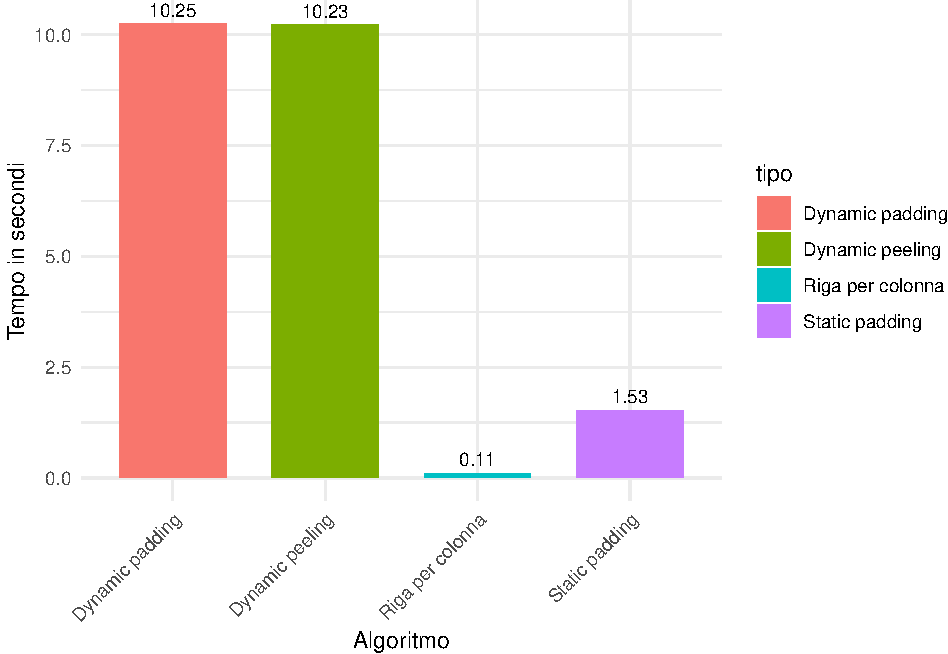
\includegraphics[width=0.48\textwidth]{figures/q_basso-1.pdf}
    \caption{Esempio di velocità media degli algoritmi con n=10.}
    \label{fig:velocità_con_Q=8}
\end{figure}

Il modo migliorare per determinare determinare il Q ottimale è in via euristica [2]. È stato quindi generato un campione con n=30. Su ogni coppia di matrici è stata testata ogni versione dell'algoritmo di Strassen per matrici rettangolari, per i valori di Q pari a $\{16,32,64,128,256,512\}$. L'algoritmo riga per colonna, invece, è stato testato solo una volta, poiché non viene influenzato dal Q. Nella Figura \ref{fig:velocità_diversi_Q} sono rappresentato i tempi di esecuzione medi per ogni Q, possiamo osservare chiaramente che le prestazioni migliori si raggiungono con Q=64 e Q=128, in particolare con Q=128 i valori sono migliori di qualche decimo di secondo, anche se non si può rilevare per via grafica. Per valori molto bassi di Q, invece, troviamo conferma del fatto che tutte e tre le versioni dell'algoritmo di Strassen sono peggiori del semplice prodotto riga per colonna. Per valori di Q maggiori di 128 invece, notiamo che le prestazioni delle tre versioni dell'algoritmo di Strassen tendono a peggiorare, ed ad avvicinarsi all'algoritmo riga per colonna. Questo avviene poiché, aumentando Q, aumenta la dimensione della matrice al più basso livello di ricorsione, che è quella su cui viene eseguito il prodotto riga per colonna.

\begin{figure}[ht]
    \centering 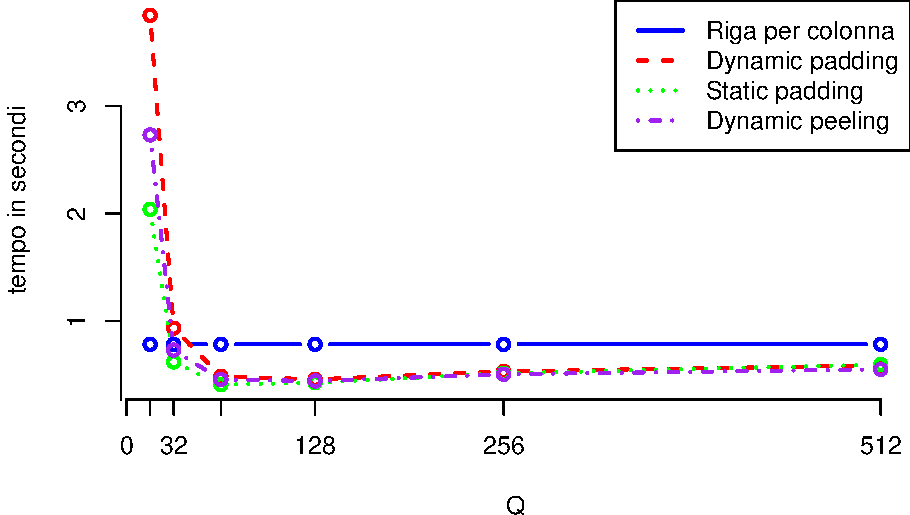
\includegraphics[width=0.48\textwidth]{figures/q_mean-1.pdf}
    \caption{Velocità media dell'algoritmo al variare di Q, n=30.}
    \label{fig:velocità_diversi_Q}
\end{figure}

Fissato quindi Q=128, confrontiamo il comportamento dei tre algoritmi di Strassen e del prodotto riga per colonna per 75 matrici di dimensioni crescenti. Grazie alla Figura \ref{fig:curva_velocità} Notiamo che al crescere del valore sulle ascisse, ossia la media geometrica di j, h e k, cresce il divario tra le tre versioni di Strassen e il prodotto riga per colonna. Inoltre possiamo notare che le versioni dell'algoritmo di Strassen hanno un comportamento quasi sovrapponibile.

\begin{figure}[ht]
    \centering 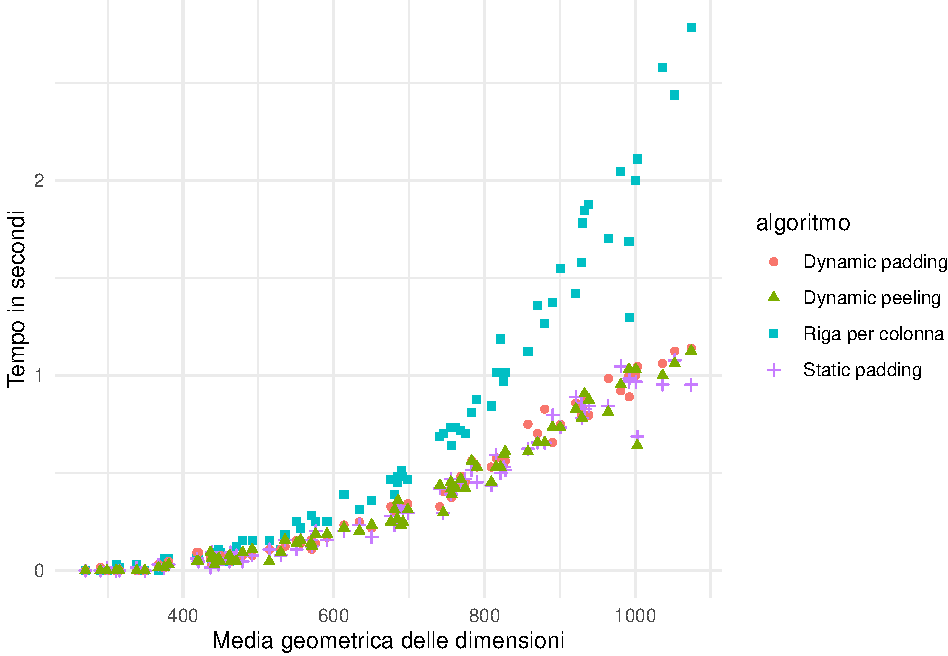
\includegraphics[width=0.48\textwidth]{figures/test_dimensioni-1.pdf}
    \caption{Confronto delle velocità su 75 coppie di matrici di dimensioni crescenti, fissato Q=128.}
    \label{fig:curva_velocità}
\end{figure}

\subsection{Sul comportamento con matrici sparse e dense}
\label{sec:sparse_vs_dense}

Un altro aspetto importante su cui soffermarsi è la diversa efficacia dei vari algoritmi in presenza di matrici sparse e dense. Per confrontarne l'efficacia sono stati generati due campioni, ciascuno con n=40. Il primo campione, quello delle matrici "dense", è stato popolato di valori interi generati in maniera casuale tra -100 e 100. Il secondo campione invece, ossia quello delle matrici "sparse", è stato popolato per metà di zeri sistematici, e per l'altra metà di valori casuali compresi tra -100 e 100. Ossia nel secondo campione almeno il 50\% delle celle era pari a 0. Successivamente, sono stati confrontati i valori medi assunti dagli algoritmi. Con l'ausilio dalla Figura \ref{fig:velocità_sparse_vs_dense}, si può notare che in entrambi i campioni le tre varianti dell'algoritmo di Strassen hanno un comportamento pressoché simile. Inoltre, notiamo che nel caso di matrice dense, le tre versioni dell'algoritmo di Strassen per matrici rettangolari sono quasi il doppio più veloci del prodotto riga per colonna. Per le matrici sparse, invece, la situazione si inverte, ossia il prodotto riga per colonna è molto più veloce dei tre algoritmi di Strassen. Infine si noti che, in entrambi i casi, tra le tre versioni dell'algoritmo di Strassen l'approccio "static padding" è quello preferibile in entrambe le situazioni.

\begin{figure}[ht]
    \centering 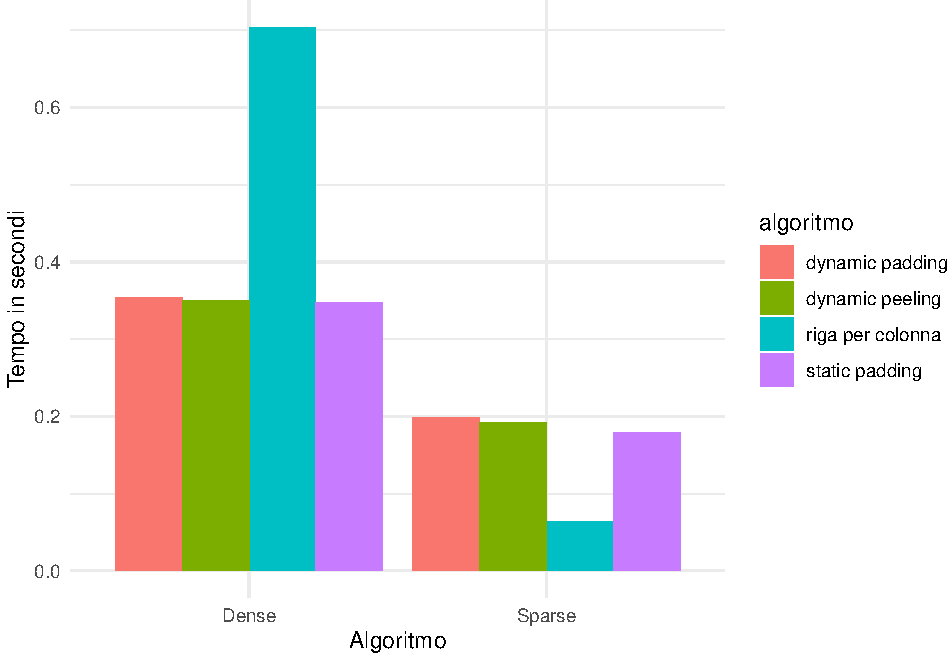
\includegraphics[width=0.48\textwidth]{figures/sparse_vs_dense-1.pdf}
    \caption{Grafico con i tempi medi di esecuzione in un campione di matrici denso e in uno di matrice sparse.}
    \label{fig:velocità_sparse_vs_dense}
\end{figure}


\subsection{Sul comportamento con matrici "lunghe" e "larghe"}

Un altro caso particolare in cui è opportuno testare l'efficacia di questi algoritmi è in presenza di matrici con numero di righe e numero di colonne fortemente sbilanciato. In particolare, definiamo come "lunga" una matrice il cui numero di righe è in media dieci volte maggiore del suo numero di colonne. Inoltre, definiamo come "larga" una matrice il cui numero di colonne è in media dieci volte maggiore del numero di righe. A questo punto prepariamo tre campioni, ciascuno con n=60. Nel primo campione A sarà larga e B generalmente rettangolare, quindi j assumerà valori tra 80 e 120, mentre h e k assumeranno valori tra 800 e 1200. Nel secondo campione invece, A sarà lunga e B sarà larga, quindi j e k assumeranno valori tra 800 e 1200, mentre h tra 80 e 120. Nel terzo campione invece, A sarà genericamente rettangolare e B sarà lunga, quindi j e h assumeranno valori tra 800 e 1200, mentre k assumerà valori tra 80 e 120. 

\begin{figure}[ht]
    \centering 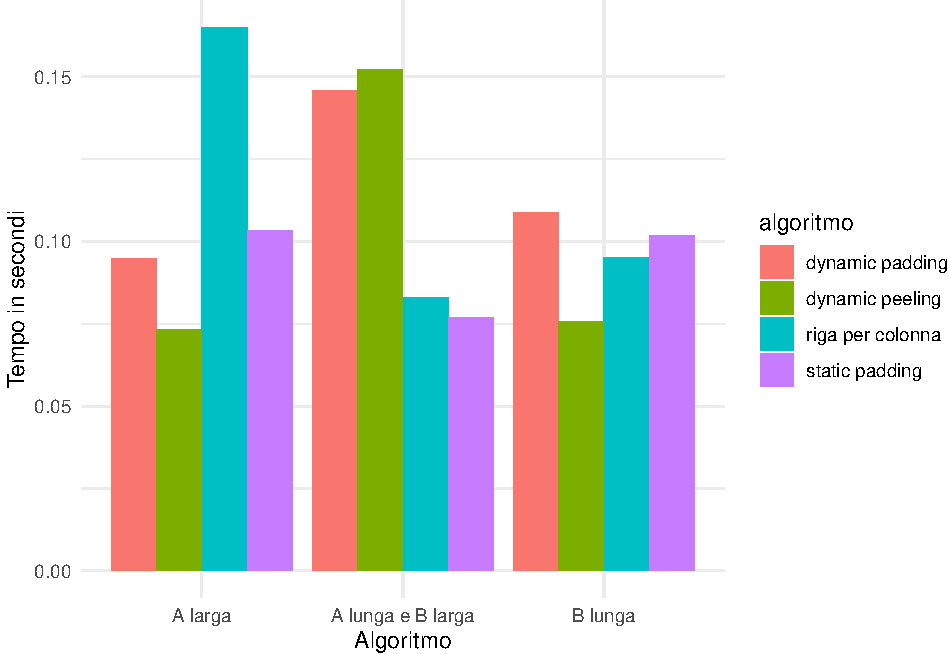
\includegraphics[width=0.48\textwidth]{figures/matrici_sbilanciate-1.pdf}
    \caption{Grafico dei valori medi dei quattro algoritmi su 3 campioni, con n=60 e Q=64.}
    \label{fig:velocità_lunghe_vs_larghe}
\end{figure}

Confrontando i tre gruppi grazie alla Figura \ref{fig:velocità_lunghe_vs_larghe}, notiamo che nel primo caso l'algoritmo riga per colonna è nettamente il più lento, mentre i tre algoritmi di Strassen hanno performance pressoché simili. Nel caso di A lunga e B larga invece, gli approcci "dynamic padding" e "dynamic peeling" sono quasi il doppio più lenti degli altri due. Nel caso di B lunga invece le performance sono pressoché uguali, ma la versione "dynamic peeling" sembra la preferibile. Globalmente la versione preferibile sembra quella "static padding", poiché è quella che rimane più costante al variare del gruppo.

In questo contesto differenti performance delle tre varianti dell'algoritmo di Strassen si potrebbero spiegare anche con le diverse scelte del criterio per il raggiungimento del cross-over point. Infatti, come evidenziato nella sezione \ref{sec:strassen_odd_matrix}, la versione "static padding" guarda solo la minima dimensione per il raggiungimento del cross-over point. Quindi nel caso di matrici in cui la dimensione minima è compresa tra 80 e 120, con Q pari a 64, il cross-over point verrà sempre raggiunto alla seconda chiamata ricorsiva. Al contrario, nel caso "dynamic padding" e "dynamic peeling" possono esserci più chiamate ricorsive, visto che per il raggiungimento del cross-over point si considera la media geometrica delle dimensioni.

\subsection{L'instabilità numerica}

Un altro punto su cui è importante testare questi algoritmi è la stabilità numerica. Prima di farlo però, è interessante notare il differente comportamento dei vari algoritmi con matrici riempite con numeri reali. Infatti confrontando un gruppo di coppie matrici riempite con numeri interi e un gruppo di coppie matrici riempite con numeri reali, ossia "floating point". Come primo gruppo prendiamo le matrici dense generate nella sezione \ref{sec:sparse_vs_dense}. Per il secondo gruppo generiamo un campione con n=40, le cui celle sono riempite con numeri casuali reali, sempre grazie alla libreria random. Grazie alla Figura \ref{fig:integer_vs_floating} possiamo notare facilmente che, in media, le matrici riempite di floating point vengono moltiplicate più velocemente dagli algoritmi. Dobbiamo però osservare che, sempre per le matrici riempite di floating point, le varie versioni dell'algoritmo di Strassen diventano più lente del classico prodotto riga per colonna.

Per quanto riguarda la stabilità numerica invece, bisogna registrare che le varie versioni dell'algoritmo di Strassen generano molti errori di approssimazione. In particolare, arrotondando le matrici C dei risultati all'ottavo numero dopo la virgola, notiamo che in media i risultati dei tre algoritmi di Strassen hanno solo il 98\% dei valori in comune con l'algoritmo riga per colonna. Questa percentuale crolla addirittura al 16\% se si arrotonda a 10 numeri dopo la virgola, e va via via peggiorando.

Nel contesto considerato quindi, emerge la conferma della non stabilità delle diverse varianti dell'algoritmo di Strassen. Tuttavia, come indicato in [2], poiché queste instabilità sono infinitesimali, possono non rappresentare un problema in molte applicazioni reali.

\begin{figure}[ht]
    \centering 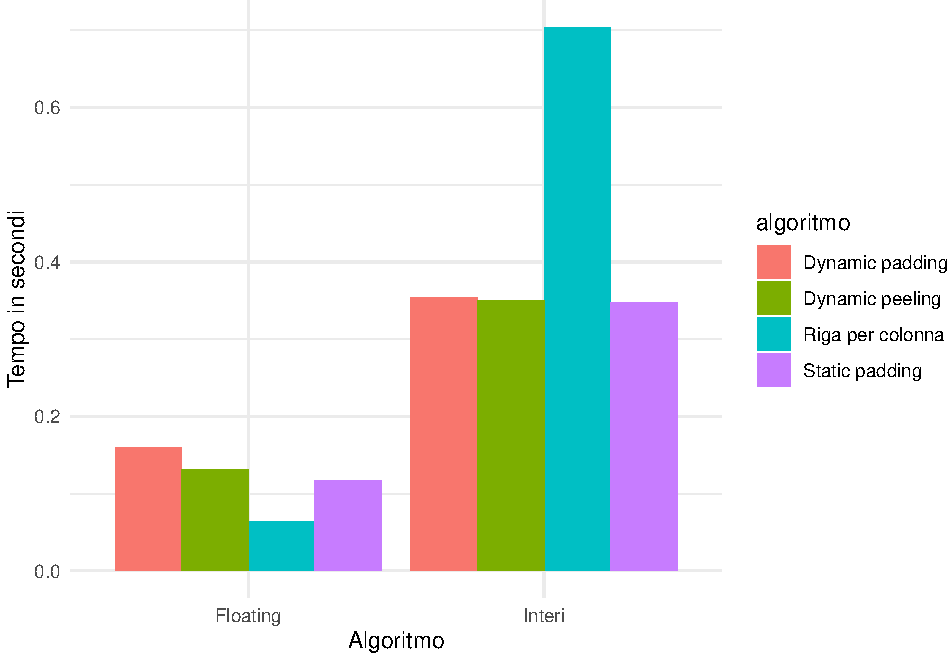
\includegraphics[width=0.48\textwidth]{figures/integer_vs_floating-1.pdf}
    \caption{Tempi media di esecuzione per matrici di interi e di floating point con i vari algoritmi, Q=128.}
    \label{fig:integer_vs_floating}
\end{figure}

\section{Conclusioni}

In conclusione i limiti di queste versioni dell'algoritmo di Strassen per matrici quadrate sono diversi. In particolare tutte le versioni non sono consigliate per matrici sparse o con floating point. Le versioni "dynamic padding" e "dynamic peeling" possono funzionare male con determinati tipi di matrici rettangolari particolarmente sbilanciati nel numero di righe e colonne. Nonostante questo, le tre versioni implementate dell'algoritmo di Strassen riescono a velocizzare il prodotto matriciale nelle altre situazioni, anche per matrici la cui media geometrica delle dimensioni è inferiore al mille. Inoltre come abbiamo osservato dalla Figura \ref{fig:curva_velocità}, l'aumento delle performance sembra crescere in maniera esponenziale al crescere delle dimensioni.  

\section{Bibliografia}

$[1]$ \textit{Gaussian Elimination is not Optimal}, Volker Strassen, Agosto 1969. \\ $[2]$ \textit{Using Strassen's Algorithm to Accelerate the Solution of Linear Systems}, David H. Bailey, King Lee, Horst D. Simon, March 1990. \\ $[3]$ \textit{Implementation of Strassen's Algorithm for Matrix Multiplication}, Steven Huss-Lederman, Elaine M. Jacobson, Jeremy R. Johnson, Anna Tsao, Thomas Turnbull, August 1996. \\ $[4]$ \textit{On the arithmetic complexity of Strassen-like matrix multiplications}, 
Murat Cenka, M. Anwar Hasan, July 2016.

\end{document}